\documentclass[border=8pt]{standalone}
\usepackage{amsmath,amssymb,bm}
\usepackage{xcolor}
\usepackage{tikz}
% --- deck palette (same values as the Part 2 slides) ---
\definecolor{P}{HTML}{4B1D8F}    % deck purple
\definecolor{band}{HTML}{F3E8FA} % soft tint for alternate multiplets
\definecolor{rule}{HTML}{CDB7E6} % light separator

\newcommand{\Kb}{\overline{K}}
% column centres (cm) and geometry
\newcommand{\cA}{2.3}\newcommand{\cB}{6.1}\newcommand{\cC}{9.0}\newcommand{\cD}{11.5}\newcommand{\cE}{13.5}
\newcommand{\Wd}{14.6}     % table width
\newcommand{\Hh}{1.3}      % header height
\newcommand{\Rh}{1.0}      % row height

% \row{i}{meson}{mass}{J^PC}{I}{S}   (i = body row, 1..10)
\newcommand{\row}[6]{%
  \pgfmathsetmacro{\yy}{-(\Hh+(#1-0.5)*\Rh)}%
  \node[text=P] at (\cA,\yy) {#2};
  \node at (\cB,\yy) {#3};
  \node at (\cC,\yy) {#4};
  \node at (\cD,\yy) {#5};
  \node at (\cE,\yy) {#6};}
% band covering rows a..b (1-based) and a separator below row b
\newcommand{\band}[2]{\fill[band] (0,{-(\Hh+(#1-1)*\Rh)}) rectangle (\Wd,{-(\Hh+#2*\Rh)});}
\newcommand{\sep}[1]{\draw[rule,line width=.6pt] (0,{-(\Hh+#1*\Rh)}) -- (\Wd,{-(\Hh+#1*\Rh)});}

\begin{document}
\Large
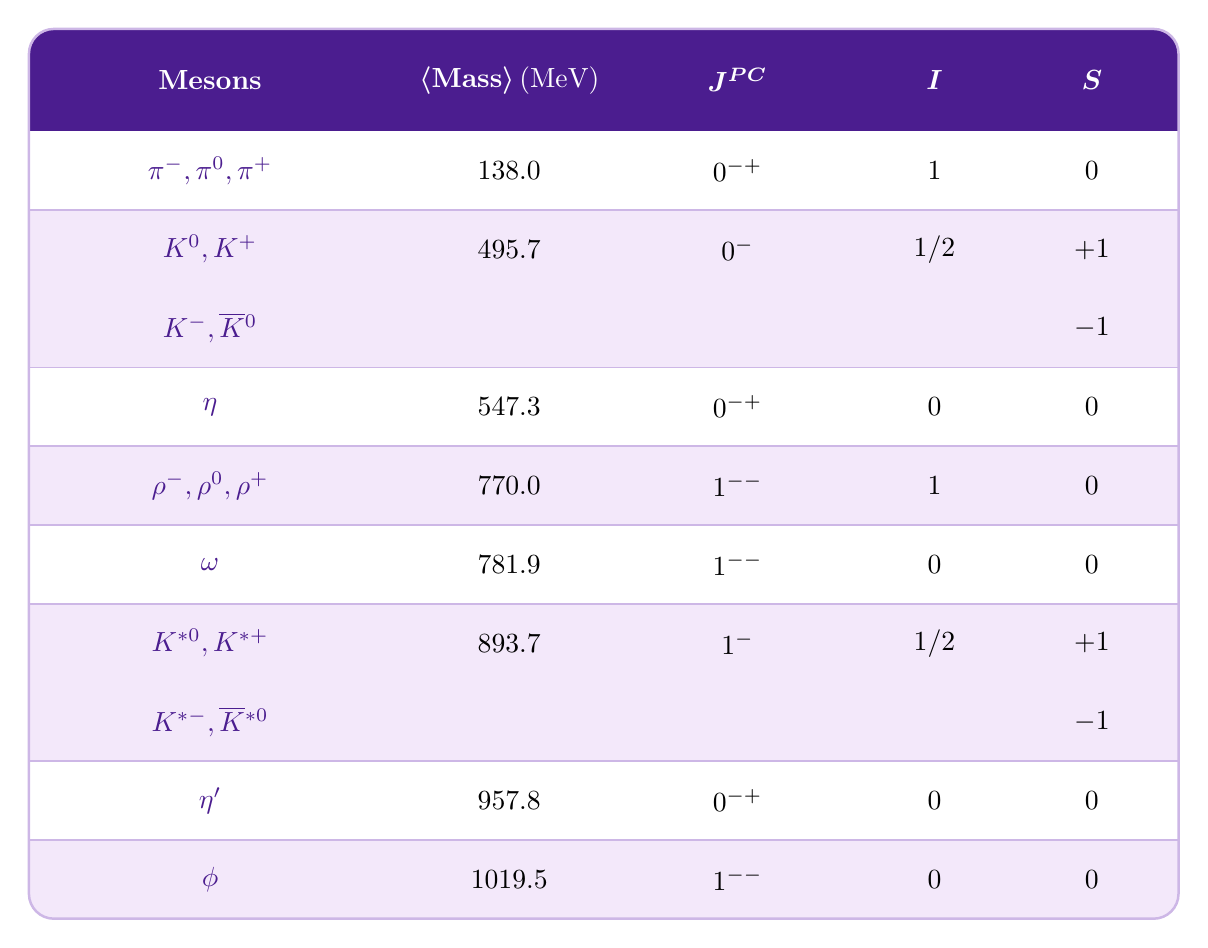
\begin{tikzpicture}
  \pgfmathsetmacro{\Ht}{\Hh+10*\Rh}
  % ---- backgrounds, clipped to a rounded rectangle ----
  \begin{scope}
    \clip[rounded corners=9pt] (0,0) rectangle (\Wd,-\Ht);
    \fill[P] (0,0) rectangle (\Wd,-\Hh);          % header bar
    \band{2}{3}\band{5}{5}\band{7}{8}\band{10}{10}% K, rho, K*, phi
  \end{scope}
  % ---- separators between multiplets ----
  \sep{1}\sep{3}\sep{4}\sep{5}\sep{6}\sep{8}\sep{9}
  \draw[rule,line width=.9pt,rounded corners=9pt] (0,0) rectangle (\Wd,-\Ht);
  % ---- header text ----
  \node[text=white] at (\cA,-\Hh/2) {\bfseries Mesons};
  \node[text=white] at (\cB,-\Hh/2) {$\bm{\langle}\textbf{Mass}\bm{\rangle}$\,{\normalsize\mdseries(MeV)}};
  \node[text=white] at (\cC,-\Hh/2) {$\bm{J^{PC}}$};
  \node[text=white] at (\cD,-\Hh/2) {$\bm{I}$};
  \node[text=white] at (\cE,-\Hh/2) {$\bm{S}$};
  % ---- body ----
  \row{1}{$\pi^-,\pi^0,\pi^+$}{$138.0$}{$0^{-+}$}{$1$}{$0$}
  \row{2}{$K^0,K^+$}{$495.7$}{$0^{-}$}{$1/2$}{$+1$}
  \row{3}{$K^-,\Kb{}^{0}$}{}{}{}{$-1$}
  \row{4}{$\eta$}{$547.3$}{$0^{-+}$}{$0$}{$0$}
  \row{5}{$\rho^-,\rho^0,\rho^+$}{$770.0$}{$1^{--}$}{$1$}{$0$}
  \row{6}{$\omega$}{$781.9$}{$1^{--}$}{$0$}{$0$}
  \row{7}{$K^{*0},K^{*+}$}{$893.7$}{$1^{-}$}{$1/2$}{$+1$}
  \row{8}{$K^{*-},\Kb{}^{*0}$}{}{}{}{$-1$}
  \row{9}{$\eta'$}{$957.8$}{$0^{-+}$}{$0$}{$0$}
  \row{10}{$\phi$}{$1019.5$}{$1^{--}$}{$0$}{$0$}
\end{tikzpicture}
\end{document}
